% !TeX spellcheck = en_US
%\documentclass[12pt]{article}

\documentclass[11pt]{report}

\usepackage[a4paper, margin=1in]{geometry}

\usepackage{mathtools}

\usepackage{listings}
\usepackage{xcolor}
\usepackage{mathtools}
\usepackage{pdfpages}
\usepackage[english]{babel}
\usepackage[labelfont=bf]{caption}
\usepackage{float}
\captionsetup{labelfont=bf}
\usepackage[normalem]{ulem}

\useunder{\uline}{\ul}{}

\definecolor{codegreen}{rgb}{0,0.6,0}
\definecolor{codegray}{rgb}{0.5,0.5,0.5}
\definecolor{codepurple}{rgb}{0.58,0,0.82}
\definecolor{backcolour}{rgb}{0.95,0.95,0.95}
\usepackage{titlesec, color}

\definecolor{gray75}{gray}{0.75}
\newcommand{\hsp}{\hspace{10pt}}
%\titleformat{\section}[hang]{\Huge\bfseries}{\thesection\hsp\textcolor{gray75}{|}\hsp}{0pt}{\Huge\bfseries}

\lstdefinestyle{mystyle}{
	backgroundcolor=\color{backcolour},   
	commentstyle=\color{codegreen},
	keywordstyle=\color{blue},
	numberstyle=\tiny\color{codegray},
	stringstyle=\color{orange},
	basicstyle=\ttfamily\footnotesize,
	breakatwhitespace=false,         
	breaklines=true,                 
	captionpos=b,                    
	keepspaces=true,                 
	numbers=left,                    
	numbersep=5pt,                  
	showspaces=false,                
	showstringspaces=false,
	showtabs=false,                  
	tabsize=2
}

\lstset{style=mystyle}

\includeonly{
	chapters/introduction,
	chapters/modeling,
	chapters/implementation,
	chapters/verification,
	chapters/simulation_experiments,
	chapters/conclusions
}

\begin{document}


\begin{titlepage}
	\begin{center}
		\begin{figure}
			
\includegraphics[width=\textwidth]{img/marchio_unipi_pant541-eps-converted-to.pdf}         
		\end{figure}
		{\Large
			Computer Engineering\\
			\vspace{5mm} %5mm vertical space
			Foundations of Cybersecurity}\\
		\vspace{30mm} %5mm vertical space
		{\Huge\textbf{\textit{secureCom}}}\\
		\vspace{10mm} %5mm vertical space
		{\Large Group Project Report}\\
		\par\noindent\rule{\textwidth}{0.4pt}
		\begin{flushright}
			\textit{TEAM MEMBERS}:\\ 
			Francesco Iemma\\
			Yuri Mazzuoli\\ 
			Olgerti Xhanej\\
			
		\end{flushright}
		\vfill
		Academic Year: 2020/2021\\        
	\end{center}
\end{titlepage} 
\tableofcontents

\chapter{How To Handle The Chat Request}
\noindent Let's start from the simple case in which a client wants to chat with another client and makes a request to the server: 
\begin{itemize}
	\item The standard channel is used to send either the request for chat and for the server's answers.
	\item If the target client accepts then the main process receive the confirmation from the server, then the main process set isChatting to true and it starts to chat.
\end{itemize}

\noindent When the server receive the command to chat with someone he has to send the chat request to the given client. Let suppose that Alice wants to chat with Bob. In this case the following steps must be performed:

\begin{itemize}
	\item The request must be done through the request channel
	\item The client daemon process (Alice's daemon process) is listening on its socket (see after) and receive the request, then it reads the variable isChatting: if it is true the daemon process refuses automatically the server request, otherwise it ask (HANDSHAKE) to the main process if he wants to speak with Bob. 
	\item The main process answer to the server by means of the daemon tools, if the answer is positive then it sets isChatting to true and so it waits for the message from Bob.
\end{itemize}

\noindent It's important to underline some concepts, first of all on the server side we have one process that handles two socket with the client, one for each channel. The protocol starts with the client that contacts the server, then the server and the client main process establish a connection and starts the protocol to establish a secure communication (Key Exchange). For standard messages this standard channel is used.

\begin{figure}[H]
	\centering
	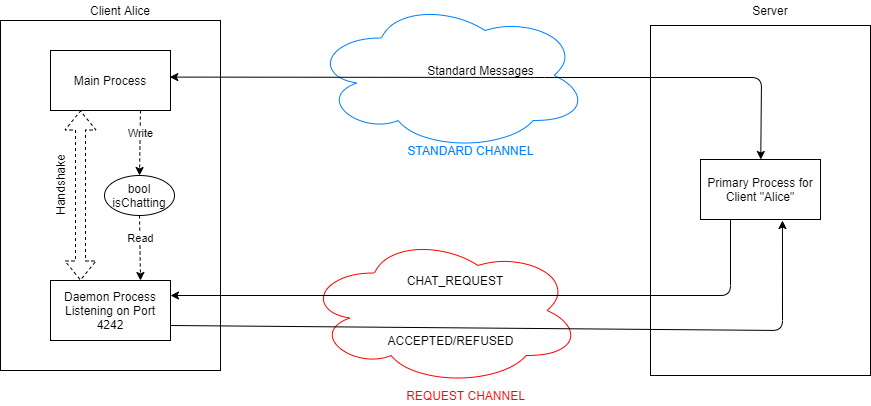
\includegraphics[scale=0.4]{img/chatRequestProtocolOneProcess.png}
	\caption{Protocol Schema}
	\label {img: chatRequestProtocolOneProcess}
\end{figure}

\noindent When the server has to sent a chat request to this client the request channel must be used. Thus it establishes a connection with the daemon process of the client that works as a server process and it is listening on port 4242 (see figure \ref{img: chatRequestProtocolOneProcess}). The security of this secondary channel is ensured by the fact that the messages sent by the server to the client on the request channel are encrypted with the shared key established during the handshake in the standard channel, hence we can say that the authentication problem is not present. In any case to implement a greater security is possible to generate client side a one time password that is sent to the server in the encrypted session through the standard channel, then the server will sent this otp to the client daemon process to identify itself.
	

\noindent Other things to take in mind are:
\begin{itemize}
	\item We assume that who send the chat request is the first to send messages.
	\item On the server side for each client two socket must be established, one for the standard channel and another one for the request channel but the process for each client is only one.
\end{itemize}


	
%	\item A third solution can be adding a command to indicate that a client is available to receive chat request. Thus:
	
%	\begin{enumerate}
%		\item A users is online when it has launched the command "available" (isChatting = false). Notice that in this case the variable isChatting can be called in a more correct way isAvailable.
		
%		\item  A users is offline (isChatting = false) if it is not available (if he has not launched the command available or if he is chatting with someone else). In that case offline means also busy whereas online means also available.
%	\end{enumerate}

	
%\end{enumerate}

%here are two possibilities:
%\begin{enumerate}
%	\item Two processes, one for the client main process and another one for the client daemon process. See figure \ref{img: chatRequestProtocolTwoProcesses}.
	
%	\begin{figure}[htpb]
%		\centering
%		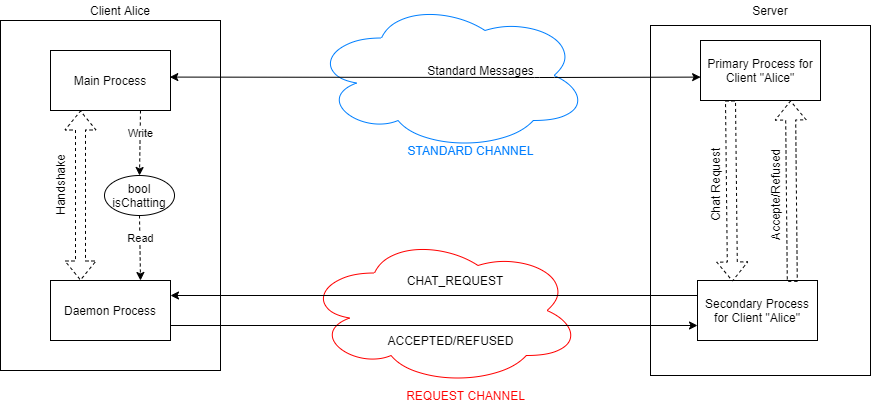
\includegraphics[scale=0.5]{img/chatRequestProtocolTwoProcesses.png}
%		\caption{Solution with two processes}
%		\label {img: chatRequestProtocolTwoProcesses}
%	\end{figure}

%\noindent Notes:


\end{document}          
